\documentclass[9ptm,twocolumn]{article}

%%% Julia %%%
\usepackage{xcolor}
    \definecolor{codegreen}{rgb}{0,0.6,0}
    \definecolor{codegray}{rgb}{0.5,0.5,0.5}
    \definecolor{codepurple}{rgb}{0.58,0,0.82}
\usepackage{listings}
\lstdefinelanguage{Julia}%
  {morekeywords={abstract,begin,break,case,catch,const,continue,do,else,elseif,%
      end,export,false,for,function,immutable,import,importall,if,in,%
      macro,module,otherwise,quote,return,switch,true,try,type,typealias,%
      using,while},%
   sensitive=true,%
   morecomment=[l]\#,%
   morecomment=[n]{\#=}{=\#},%
   morestring=[s]{"}{"},%
   morestring=[m]{'}{'},%
}[keywords,comments,strings]%

\lstdefinestyle{mystyle}{
    commentstyle=\color{codegreen},
    keywordstyle=\color{magenta},
    stringstyle=\color{codepurple},
    basicstyle=\ttfamily\footnotesize,
    breakatwhitespace=false,
    breaklines=true,
    captionpos=b,
    keepspaces=true,
    showspaces=false,
    showstringspaces=false,
    showtabs=false,
    tabsize=2
}
\lstset{style=mystyle}
%%%%%%%%%%%%%

\usepackage{hyperref}
\usepackage{lipsum}
\usepackage{tikz}
\usetikzlibrary{external}
%\tikzexternalize[prefix=figures/] % Folder in which files are saved. Uncomment to externalize

\usepackage{pgfplots}
\pgfplotsset{compat=newest}
  \usetikzlibrary{plotmarks}
  \usetikzlibrary{arrows.meta}
  \usepgfplotslibrary{patchplots}

\title{PGFPlots example using Julia}
\author{Karel Mundnich}
\date{}

\begin{document}
\maketitle
\tikzexternaldisable

\section{Introduction}
The figures in this document have been generated with the Julia \texttt{Plots.jl} package using the \texttt{pgfplots()} backend. The following code allows to create the TikZ figures:
\begin{lstlisting}[language=Julia]
using CSV
using Plots; pgfplots()
using DataFrames

df = DataFrame(
	x = 1:10,
	y1 = 1:10,
	y2 = (1:10).^2
	)
plot(df.x, df.y1)
plot!(df.x, df.y2)

savefig("tikz/example_figure.tex")
CSV.write("data/data.csv", df)
\end{lstlisting}

To include the figure into the text, we load the following packages in the preamble:
\begin{verbatim}
\usepackage{tikz}
\usetikzlibrary{external}
% \tikzexternalize[prefix=figures/]

\usepackage{pgfplots}
\pgfplotsset{compat=newest}
  \usetikzlibrary{plotmarks}
  \usetikzlibrary{arrows.meta}
  \usepgfplotslibrary{patchplots}
\end{verbatim}
\texttt{\\tikzexternalize[prefix=figures/]} includes the folder where the figures are saved after TikZ externalization.

To load a figure, we use the following \LaTeX code:

\begin{verbatim}
\begin{figure}
\centering
\tikzsetnextfilename{example_figure}
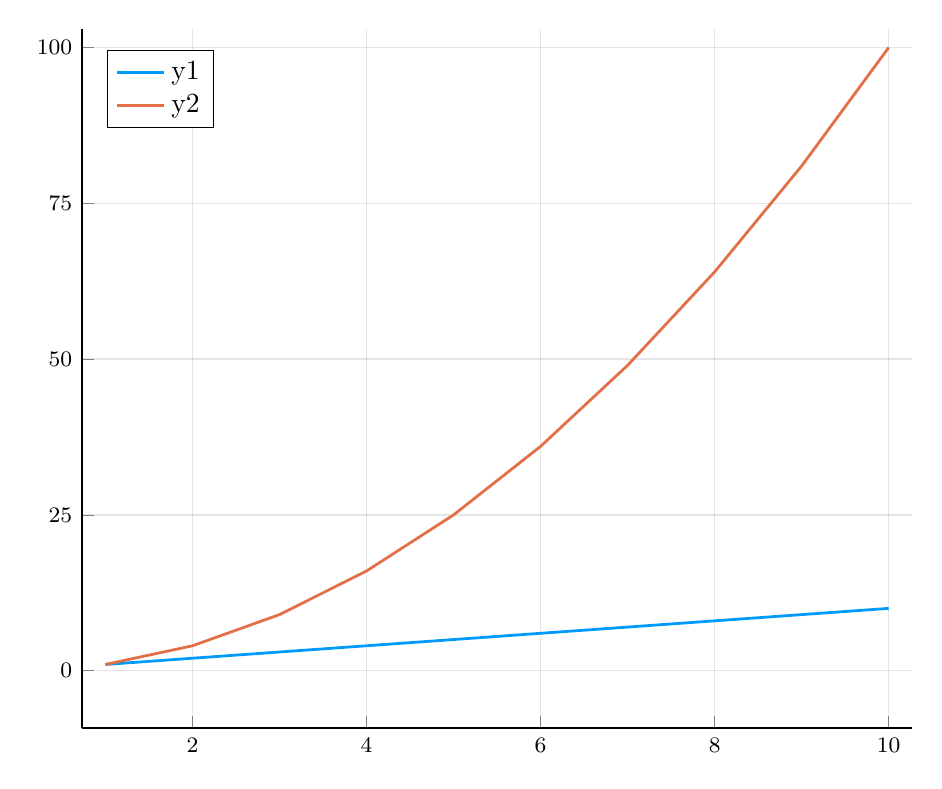
\begin{tikzpicture}[]
\begin{axis}[
    width = \columnwidth,
    ylabel = {},
    xmin = {0.73},
    xmax = {10.27},
    ymax = {102.97},
    xlabel = {},
    unbounded coords=jump,
    scaled x ticks = false,
    xlabel style = {font = {\fontsize{11 pt}{14.3 pt}\selectfont}, color = {rgb,1:red,0.00000000;green,0.00000000;blue,0.00000000}, draw opacity = 1.0, rotate = 0.0},
    xmajorgrids = true,
    xtick = {2.0,4.0,6.0,8.0,10.0},
    xticklabels = {$2$,$4$,$6$,$8$,$10$},
    xtick align = inside,
    xticklabel style = {
        font = {\fontsize{8 pt}{10.4 pt}\selectfont},
        color = {rgb,1:red,0.00000000;green,0.00000000;blue,0.00000000},
        draw opacity = 1.0,
        rotate = 0.0},
    x grid style = {
        color = {rgb,1:red,0.00000000;green,0.00000000;blue,0.00000000},
        draw opacity = 0.1,
        line width = 0.5,
        solid},
    axis x line* = left,
    x axis line style = {
        color = {rgb,1:red,0.00000000;green,0.00000000;blue,0.00000000},
        draw opacity = 1.0,
        line width = 1,
        solid},
    scaled y ticks = false,
    ylabel style = {
        font = {\fontsize{11 pt}{14.3 pt}\selectfont},
        color = {rgb,1:red,0.00000000;green,0.00000000;blue,0.00000000},
        draw opacity = 1.0,
        rotate = 0.0},
    ymajorgrids = true,
    ytick = {0.0,25.0,50.0,75.0,100.0},
    yticklabels = {$0$,$25$,$50$,$75$,$100$},
    ytick align = inside,
    yticklabel style = {font = {\fontsize{8 pt}{10.4 pt}\selectfont},
    color = {rgb,1:red,0.00000000;green,0.00000000;blue,0.00000000},
    draw opacity = 1.0, rotate = 0.0},
    y grid style = {
        color = {rgb,1:red,0.00000000;green,0.00000000;blue,0.00000000},
        draw opacity = 0.1,
        line width = 0.5,
        solid},
    axis y line* = left,
    y axis line style = {color = {rgb,1:red,0.00000000;green,0.00000000;blue,0.00000000},
        draw opacity = 1.0,
        line width = 1,
        solid},
    xshift = 0.0mm,
    yshift = 0.0mm,
    axis background/.style={fill={rgb,1:red,1.00000000;green,1.00000000;blue,1.00000000}},
    legend pos = {north west}
]

\addplot+ [
    color = {rgb,1:red,0.00000000;green,0.60560316;blue,0.97868012},
    draw opacity = 1.0,
    line width = 1,
    solid,
    mark = none,
    mark size = 2.0,
    mark options = {
            color = {rgb,1:red,0.00000000;green,0.00000000;blue,0.00000000}, draw opacity = 1.0,
            fill = {rgb,1:red,0.00000000;green,0.60560316;blue,0.97868012}, fill opacity = 1.0,
            line width = 1,
            rotate = 0,
            solid
        }] coordinates {
(1.0, 1.0)
(2.0, 2.0)
(3.0, 3.0)
(4.0, 4.0)
(5.0, 5.0)
(6.0, 6.0)
(7.0, 7.0)
(8.0, 8.0)
(9.0, 9.0)
(10.0, 10.0)
};
\addlegendentry{y1}
\addplot+ [
    color = {rgb,1:red,0.88887350;green,0.43564919;blue,0.27812294},
    draw opacity = 1.0,
    line width = 1,
    solid,mark = none,
    mark size = 2.0,
    mark options = {
            color = {rgb,1:red,0.00000000;green,0.00000000;blue,0.00000000}, draw opacity = 1.0,
            fill = {rgb,1:red,0.88887350;green,0.43564919;blue,0.27812294}, fill opacity = 1.0,
            line width = 1,
            rotate = 0,
            solid
        }]coordinates {
(1.0, 1.0)
(2.0, 4.0)
(3.0, 9.0)
(4.0, 16.0)
(5.0, 25.0)
(6.0, 36.0)
(7.0, 49.0)
(8.0, 64.0)
(9.0, 81.0)
(10.0, 100.0)
};
\addlegendentry{y2}
\end{axis}

\end{tikzpicture}

\end{figure}
\end{verbatim}

This generates Figure~\ref{fig:example}.

\begin{figure}
\centering
\tikzsetnextfilename{example_figure}
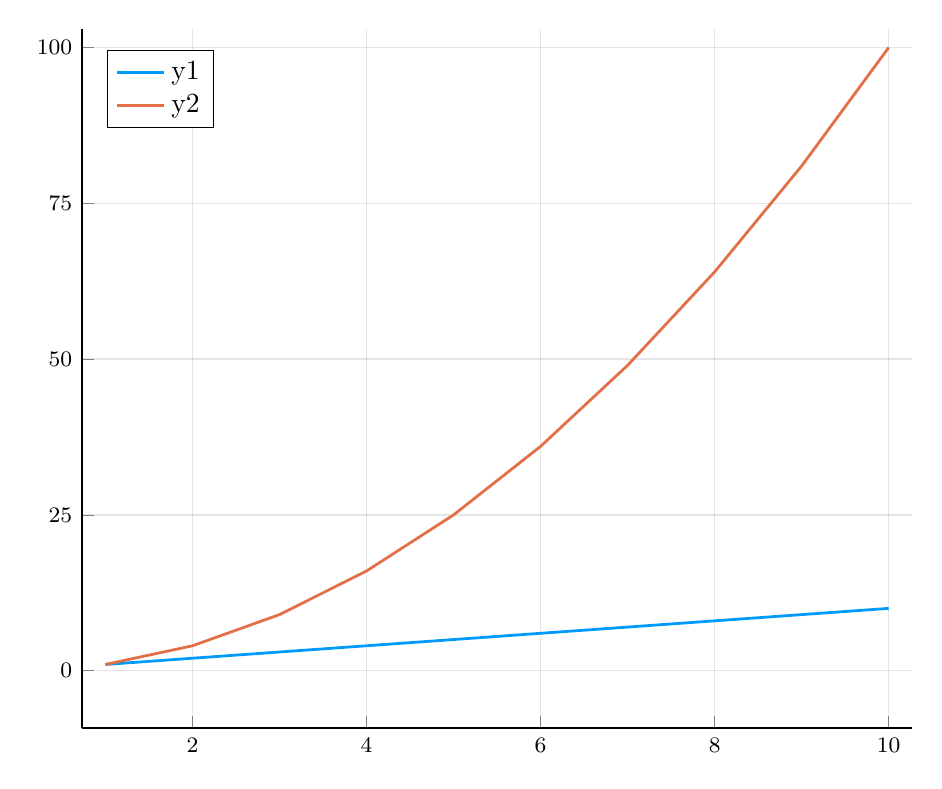
\begin{tikzpicture}[]
\begin{axis}[
    width = \columnwidth,
    ylabel = {},
    xmin = {0.73},
    xmax = {10.27},
    ymax = {102.97},
    xlabel = {},
    unbounded coords=jump,
    scaled x ticks = false,
    xlabel style = {font = {\fontsize{11 pt}{14.3 pt}\selectfont}, color = {rgb,1:red,0.00000000;green,0.00000000;blue,0.00000000}, draw opacity = 1.0, rotate = 0.0},
    xmajorgrids = true,
    xtick = {2.0,4.0,6.0,8.0,10.0},
    xticklabels = {$2$,$4$,$6$,$8$,$10$},
    xtick align = inside,
    xticklabel style = {
        font = {\fontsize{8 pt}{10.4 pt}\selectfont},
        color = {rgb,1:red,0.00000000;green,0.00000000;blue,0.00000000},
        draw opacity = 1.0,
        rotate = 0.0},
    x grid style = {
        color = {rgb,1:red,0.00000000;green,0.00000000;blue,0.00000000},
        draw opacity = 0.1,
        line width = 0.5,
        solid},
    axis x line* = left,
    x axis line style = {
        color = {rgb,1:red,0.00000000;green,0.00000000;blue,0.00000000},
        draw opacity = 1.0,
        line width = 1,
        solid},
    scaled y ticks = false,
    ylabel style = {
        font = {\fontsize{11 pt}{14.3 pt}\selectfont},
        color = {rgb,1:red,0.00000000;green,0.00000000;blue,0.00000000},
        draw opacity = 1.0,
        rotate = 0.0},
    ymajorgrids = true,
    ytick = {0.0,25.0,50.0,75.0,100.0},
    yticklabels = {$0$,$25$,$50$,$75$,$100$},
    ytick align = inside,
    yticklabel style = {font = {\fontsize{8 pt}{10.4 pt}\selectfont},
    color = {rgb,1:red,0.00000000;green,0.00000000;blue,0.00000000},
    draw opacity = 1.0, rotate = 0.0},
    y grid style = {
        color = {rgb,1:red,0.00000000;green,0.00000000;blue,0.00000000},
        draw opacity = 0.1,
        line width = 0.5,
        solid},
    axis y line* = left,
    y axis line style = {color = {rgb,1:red,0.00000000;green,0.00000000;blue,0.00000000},
        draw opacity = 1.0,
        line width = 1,
        solid},
    xshift = 0.0mm,
    yshift = 0.0mm,
    axis background/.style={fill={rgb,1:red,1.00000000;green,1.00000000;blue,1.00000000}},
    legend pos = {north west}
]

\addplot+ [
    color = {rgb,1:red,0.00000000;green,0.60560316;blue,0.97868012},
    draw opacity = 1.0,
    line width = 1,
    solid,
    mark = none,
    mark size = 2.0,
    mark options = {
            color = {rgb,1:red,0.00000000;green,0.00000000;blue,0.00000000}, draw opacity = 1.0,
            fill = {rgb,1:red,0.00000000;green,0.60560316;blue,0.97868012}, fill opacity = 1.0,
            line width = 1,
            rotate = 0,
            solid
        }] coordinates {
(1.0, 1.0)
(2.0, 2.0)
(3.0, 3.0)
(4.0, 4.0)
(5.0, 5.0)
(6.0, 6.0)
(7.0, 7.0)
(8.0, 8.0)
(9.0, 9.0)
(10.0, 10.0)
};
\addlegendentry{y1}
\addplot+ [
    color = {rgb,1:red,0.88887350;green,0.43564919;blue,0.27812294},
    draw opacity = 1.0,
    line width = 1,
    solid,mark = none,
    mark size = 2.0,
    mark options = {
            color = {rgb,1:red,0.00000000;green,0.00000000;blue,0.00000000}, draw opacity = 1.0,
            fill = {rgb,1:red,0.88887350;green,0.43564919;blue,0.27812294}, fill opacity = 1.0,
            line width = 1,
            rotate = 0,
            solid
        }]coordinates {
(1.0, 1.0)
(2.0, 4.0)
(3.0, 9.0)
(4.0, 16.0)
(5.0, 25.0)
(6.0, 36.0)
(7.0, 49.0)
(8.0, 64.0)
(9.0, 81.0)
(10.0, 100.0)
};
\addlegendentry{y2}
\end{axis}

\end{tikzpicture}

% \includegraphics{figures/example_figure.pdf}
\caption{This is an example figure using PGFPlots.}
\label{fig:example}
\end{figure}

\section{Figure sizes}
Figure~\ref{fig:example} is loaded from \texttt{tikz/example\_figure.tex}. This figure has been formatted by hand for clarity. The second figure is a copy of the first figure, where the width has been changed intentionally.

Note that in the first figure, we use:
\begin{verbatim}
width=\columnwidth,	
\end{verbatim}
while in the second figure, we use:
\begin{verbatim}
width=\textwidth,	
\end{verbatim}
to set the width of the figures. When setting the size of the figures, it is important to note the effect of the command \texttt{scale axis only}. If using this command in the \texttt{axis} properties, then the \texttt{width} and \texttt{height} values only scale the axes, but do not consider the space used by labels and ticks.


\section{Loading the data from a \\separate file}
The dataframe generated in Julia has been saved to \texttt{data/data.tex}. Note that this file has been used in Figure~\ref{fig:example_modified} to load the data, but not in Figure~\ref{fig:example}. Loading the data from a file allows the reuse of the TikZ code without the need to change the figures over and over. Moreover, figure templates can be generated for reuse!

\section{Saving the figures as PDF files}
To save the figures to PDF files, one may use the TikZ \texttt{external} library (included in the \LaTeX code in the Introduction). In this document, we have used the commands \texttt{tikzexternalenable} and \texttt{tikzexternaldisable} to selectively externalize Figure~\ref{fig:example_modified} and not Figure~\ref{fig:example}.

To externalize, we first uncomment the following line in the preamble:
\begin{verbatim}
% \tikzexternalize[prefix=figures/]
\end{verbatim}
and then compile the document using the following from the command line:
\begin{verbatim}
$ pdflatex --shell-escape main.tex
\end{verbatim}
Note that \texttt{xelatex} and \texttt{lualatex} may be used as well. When finished, we will find a PDF version of the externalized figures in the \texttt{figures/} folder. We can load this figure using \texttt{includegraphics} command, as with any other regular figure.

\section{Filler text}

\lipsum[2-3]



\lipsum[4]

\begin{figure*}
\centering
\tikzexternalenable % We externalize *only* this figure
\tikzsetnextfilename{example_figure_modified} % Saved in figures/example_figure_modified.pdf
%\begin{tikzpicture}[]
\begin{axis}[
    width = \textwidth,
    height = 0.3\textwidth,
    ylabel = {},
    xmin = {0.73},
    xmax = {10.27},
    ymax = {102.97},
    xlabel = {},
    unbounded coords=jump,
    scaled x ticks = false,
    xlabel style = {font = {\fontsize{11 pt}{14.3 pt}\selectfont}, color = {rgb,1:red,0.00000000;green,0.00000000;blue,0.00000000}, draw opacity = 1.0, rotate = 0.0},
    xmajorgrids = true,
    xtick = {2.0,4.0,6.0,8.0,10.0},
    xticklabels = {$2$,$4$,$6$,$8$,$10$},
    xtick align = inside,
    xticklabel style = {
        font = {\fontsize{8 pt}{10.4 pt}\selectfont},
        color = {rgb,1:red,0.00000000;green,0.00000000;blue,0.00000000},
        draw opacity = 1.0,
        rotate = 0.0},
    x grid style = {
        color = {rgb,1:red,0.00000000;green,0.00000000;blue,0.00000000},
        draw opacity = 0.1,
        line width = 0.5,
        solid},
    axis x line* = left,
    x axis line style = {
        color = {rgb,1:red,0.00000000;green,0.00000000;blue,0.00000000},
        draw opacity = 1.0,
        line width = 1,
        solid},
    scaled y ticks = false,
    ylabel style = {
        font = {\fontsize{11 pt}{14.3 pt}\selectfont},
        color = {rgb,1:red,0.00000000;green,0.00000000;blue,0.00000000},
        draw opacity = 1.0,
        rotate = 0.0},
    ymajorgrids = true,
    ytick = {0.0,25.0,50.0,75.0,100.0},
    yticklabels = {$0$,$25$,$50$,$75$,$100$},
    ytick align = inside,
    yticklabel style = {font = {\fontsize{8 pt}{10.4 pt}\selectfont},
    color = {rgb,1:red,0.00000000;green,0.00000000;blue,0.00000000},
    draw opacity = 1.0, rotate = 0.0},
    y grid style = {
        color = {rgb,1:red,0.00000000;green,0.00000000;blue,0.00000000},
        draw opacity = 0.1,
        line width = 0.5,
        solid},
    axis y line* = left,
    y axis line style = {color = {rgb,1:red,0.00000000;green,0.00000000;blue,0.00000000},
        draw opacity = 1.0,
        line width = 1,
        solid},
    xshift = 0.0mm,
    yshift = 0.0mm,
    axis background/.style={fill={rgb,1:red,1.00000000;green,1.00000000;blue,1.00000000}},
    legend pos = {north west}
]

\addplot+ [
    color = {rgb,1:red,0.00000000;green,0.60560316;blue,0.97868012},
    draw opacity = 1.0,
    line width = 1,
    solid,
    mark = none,
    mark size = 2.0,
    mark options = {
            color = {rgb,1:red,0.00000000;green,0.00000000;blue,0.00000000}, draw opacity = 1.0,
            fill = {rgb,1:red,0.00000000;green,0.60560316;blue,0.97868012}, fill opacity = 1.0,
            line width = 1,
            rotate = 0,
            solid
        }] table [x = x, y = y1, col sep = comma] {data/data.csv};
\addlegendentry{y1}
\addplot+ [
    color = {rgb,1:red,0.88887350;green,0.43564919;blue,0.27812294},
    draw opacity = 1.0,
    line width = 1,
    solid,mark = none,
    mark size = 2.0,
    mark options = {
            color = {rgb,1:red,0.00000000;green,0.00000000;blue,0.00000000}, draw opacity = 1.0,
            fill = {rgb,1:red,0.88887350;green,0.43564919;blue,0.27812294}, fill opacity = 1.0,
            line width = 1,
            rotate = 0,
            solid
        }] table[x = x, y = y2, col sep = comma] {data/data.csv};
\addlegendentry{y2}
\end{axis}

\end{tikzpicture}
 % Comment after externalizing
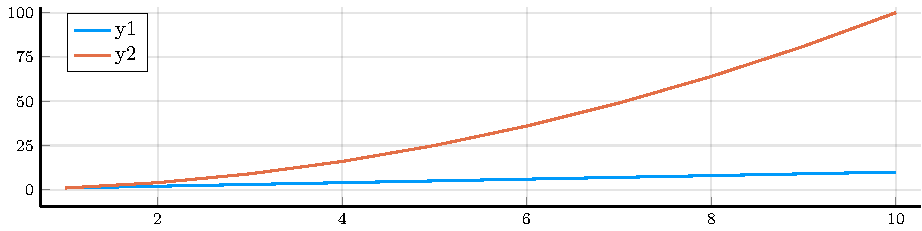
\includegraphics{figures/example_figure_modified.pdf} % Uncomment after externalizing
\caption{This is a modified example of Figure~\ref{fig:example}.}
\label{fig:example_modified}
\tikzexternaldisable
\end{figure*}

\lipsum[5-12]


\end{document}